% !TeX root = ../main.tex
% Borrador preparado para sustituir el bloque 6.3 de sections/implementacion.tex.
% Se mantiene separado para revisión antes de integrar en el capítulo completo.

\subsection{Implementación de la sonificación}

La sonificación constituye la tercera capa ejecutable de la cadena EEG--MIDI. Su entrada no son muestras crudas ni ventanas temporales de señal, sino el resultado ya producido por el backend descrito en la sección anterior: características espectrales, diagnósticos observacionales y estado de calidad de la ventana. A partir de esta representación intermedia, el sistema construye controles musicales normalizados, genera una estructura musical jerárquica y finalmente programa mensajes MIDI para la salida física.

La ruta implementada evita una traducción directa de una banda EEG a una nota concreta. En su lugar, el sistema separa tres tipos de información: las características derivadas del EEG, la evaluación de calidad de la ventana y la configuración musical elegida por el usuario o fijada por el backend. Con esta separación, el EEG modula variables como actividad, densidad, registro, estabilidad, dinámica y probabilidad de nota, mientras que elementos como la escala, la nota raíz, la nota principal, el canal MIDI y el programa se mantienen como parámetros musicales de configuración.

La Figura~\ref{fig:impl_sonificacion_flujo} resume el flujo principal implementado. La figura debe leerse como continuación directa de la sección 6.2: el bloque DSP y el \textit{quality gate} ya han producido sus salidas, y la sonificación comienza en \texttt{SonificationFeatureAdapter}.

\begin{figure}[H]
    \centering
    \IfFileExists{images/uml/impl_sonificacion_flujo.png}{%
        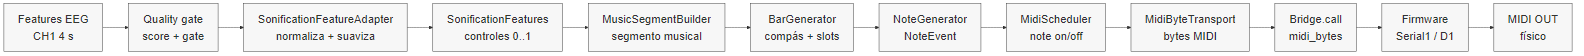
\includegraphics[width=0.98\textwidth,height=0.42\textheight,keepaspectratio]{images/uml/impl_sonificacion_flujo.png}
    }{%
        \IfFileExists{images/uml/impl_sonificacion_flujo.pdf}{%
            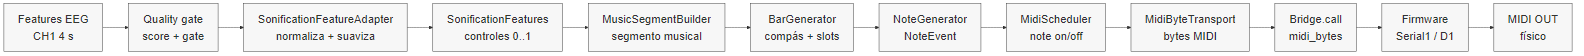
\includegraphics[width=0.98\textwidth,height=0.42\textheight,keepaspectratio]{images/uml/impl_sonificacion_flujo.pdf}
        }{%
            \fbox{\parbox{0.9\textwidth}{\centering Diagrama pendiente de exportar desde Mermaid: \texttt{images/uml/impl\_sonificacion\_flujo.mmd}}}%
        }%
    }
    \caption{Flujo principal de sonificación implementado. Las características EEG y la calidad de señal se transforman en controles musicales, después en segmentos, compases, notas y finalmente en eventos MIDI enviados al firmware mediante \texttt{midi\_bytes}.}
    \label{fig:impl_sonificacion_flujo}
\end{figure}

\subsubsection{Segmentación EEG}

En esta sección, el término segmentación no se refiere a una segmentación \textit{offline} de registros EEG ni a la detección clínica de estados cerebrales. La implementación trabaja sobre la ventana viva ya calculada por el backend: CH1 se analiza en ventanas de \SI{4}{\second}, actualizadas cada 64 muestras, y el resultado de esa ventana se entrega a la sonificación como un diccionario de características. Por tanto, el primer paso de 6.3 consiste en transformar una ventana EEG ya resumida en controles musicales, no en volver a procesar la señal temporal.

El módulo \texttt{sonification\_features.py} concentra esta frontera. Su documentación interna establece explícitamente que no calcula DSP, no importa \texttt{EEGSignalProcessor} y no depende de \texttt{BackendService}; recibe el diccionario ya calculado por \texttt{compute\_live\_features()} y lo convierte en una estructura \texttt{SonificationFeatures}. Esta decisión mantiene la separación de responsabilidades: el cálculo espectral pertenece a 6.2, mientras que 6.3 empieza con una representación musicalmente utilizable de esas características.

La clase \texttt{SonificationFeatures} agrupa controles normalizados en el intervalo \([0,1]\). Estos controles son reportables en el \textit{snapshot}, en la WebUI, en capturas y en la memoria del TFG. Los principales son \texttt{alpha\_drive}, \texttt{beta\_gamma\_drive}, \texttt{rms\_beta\_activity}, \texttt{band\_driven\_density}, \texttt{spectral\_register}, \texttt{alpha\_stability}, \texttt{rms\_band\_velocity} y \texttt{band\_note\_probability}. El objeto conserva además información trazable, como RMS en voltios y microvoltios, frecuencia pico, banda dominante y potencias por banda.

La Tabla~\ref{tab:impl_sonificacion_controles} resume el significado de estos controles dentro del motor musical. Esta tabla no debe interpretarse como una tabla clínica de bandas EEG, sino como una descripción del mapeo algorítmico utilizado para generar música.

\begin{table}[H]
    \centering
    \caption{Controles principales usados por la sonificación.}
    \label{tab:impl_sonificacion_controles}
    \renewcommand{\arraystretch}{1.15}
    \begin{tabular}{p{0.23\textwidth}p{0.25\textwidth}p{0.28\textwidth}p{0.14\textwidth}}
        \hline
        \textbf{Control} & \textbf{Origen EEG} & \textbf{Interpretación musical} & \textbf{Rango/efecto} \\
        \hline
        \texttt{alpha\_drive} & Relación relativa entre alfa y beta & Tendencia a estabilidad o reposo musical & 0--1 \\
        \texttt{beta\_gamma\_drive} & Peso de beta y gamma & Tensión, síncopa o actividad rápida & 0--1 \\
        \texttt{rms\_beta\_activity} & RMS normalizado combinado con beta/gamma & Actividad global del compás & 0--1 \\
        \texttt{band\_driven\_density} & Densidad derivada de bandas rápidas y RMS & Cantidad de eventos rítmicos & 0--1 \\
        \texttt{spectral\_register} & Frecuencia pico y peso de bandas rápidas & Desplazamiento hacia registro grave/agudo & 0--1 \\
        \texttt{alpha\_stability} & Alfa, theta y nivel RMS & Estabilidad armónica relativa & 0--1 \\
        \texttt{rms\_band\_velocity} & RMS y bandas rápidas & Dinámica o \textit{velocity} MIDI & 0--1 \\
        \texttt{band\_note\_probability} & Densidad espectral musicalizada & Probabilidad de activar notas & 0--1 \\
        \texttt{quality\_gate} & Estado de calidad espectral & Atenuación o bloqueo musical & 0--1 \\
        \hline
    \end{tabular}
\end{table}

El \texttt{quality\_gate} se incorpora a la sonificación antes de generar nuevo material musical. Si la calidad de la ventana es alta, los controles se aplican con normalidad; si la ventana presenta artefactos o baja fiabilidad, los controles sensibles se atenúan. En particular, la implementación reduce la actividad, la densidad, la velocidad y la probabilidad de nota cuando el factor de puerta disminuye. Si no existen características válidas o el \textit{score} cae por debajo del umbral de uso, la sonificación deja de generar nuevo material útil hasta recibir una ventana posterior válida.

La Figura~\ref{fig:impl_sonificacion_quality_gate} muestra esta relación entre características, diagnósticos, calidad y controles musicales. La finalidad de la figura es aclarar que la calidad no modifica la adquisición ni recalcula el DSP, sino que actúa como una puerta entre las características EEG y el motor musical.

\begin{figure}[H]
    \centering
    \IfFileExists{images/uml/impl_sonificacion_quality_gate.png}{%
        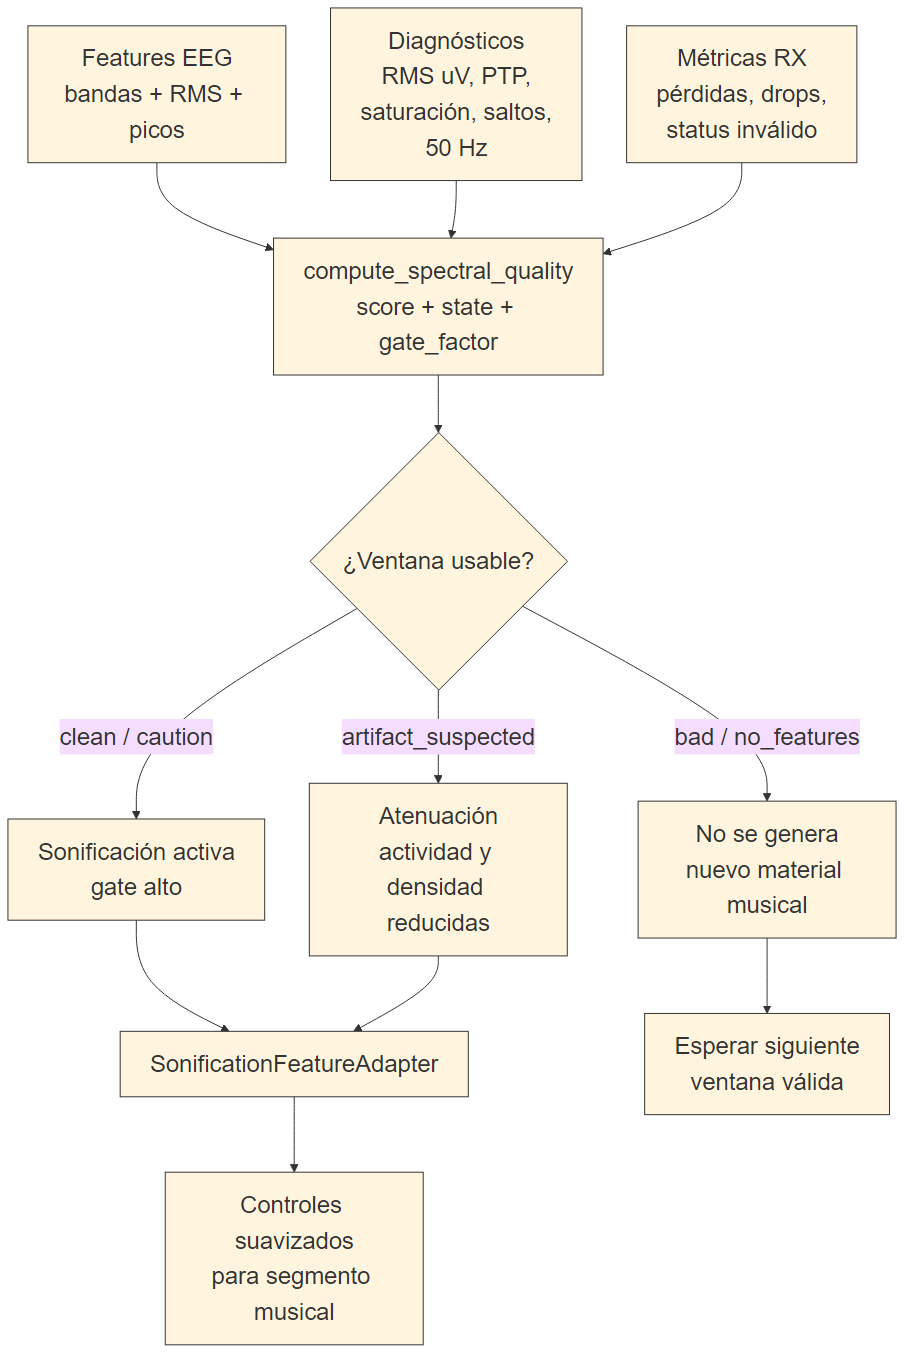
\includegraphics[width=0.95\textwidth,height=0.42\textheight,keepaspectratio]{images/uml/impl_sonificacion_quality_gate.png}
    }{%
        \IfFileExists{images/uml/impl_sonificacion_quality_gate.pdf}{%
            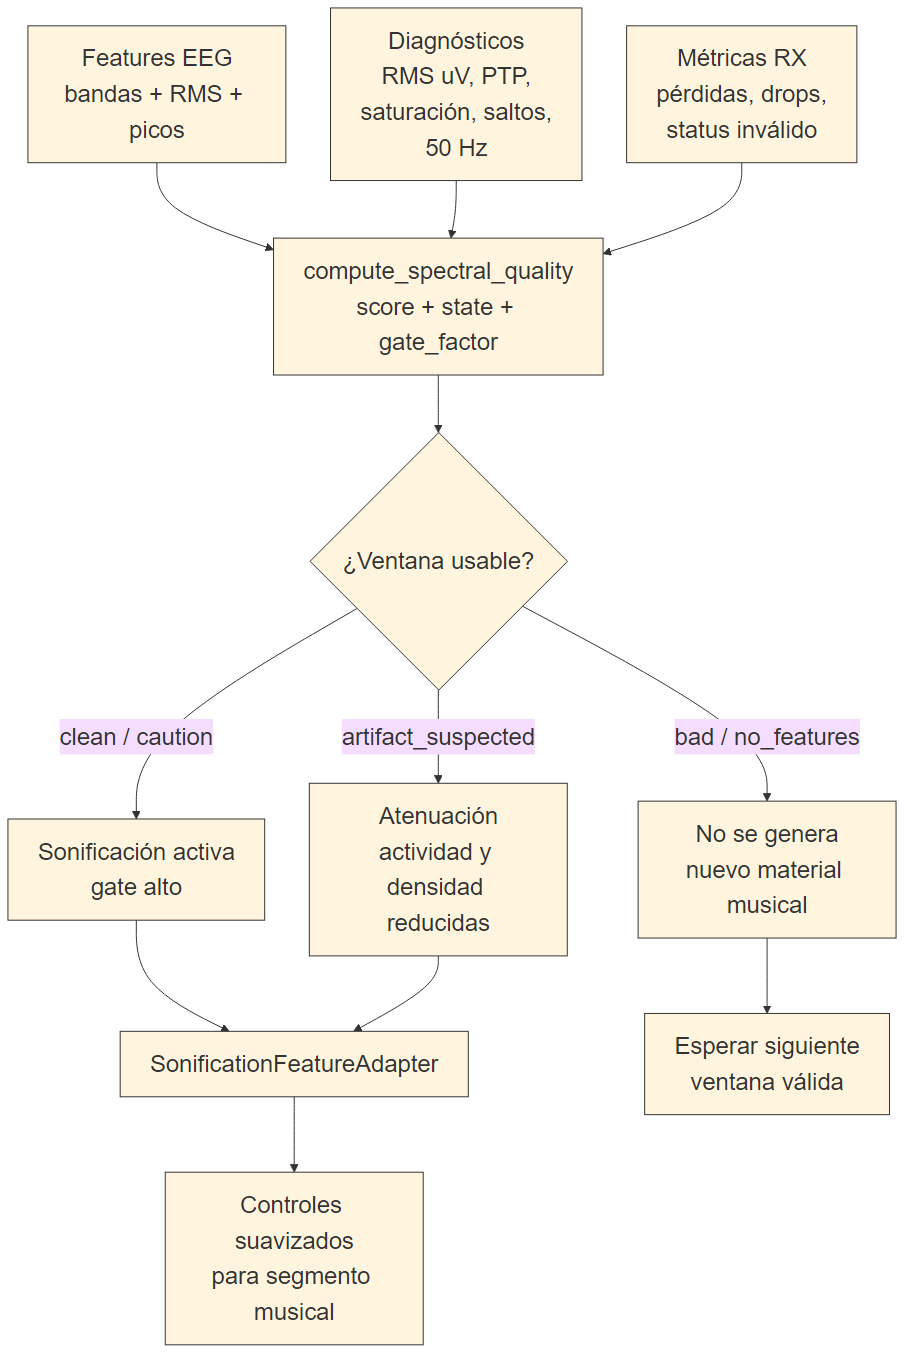
\includegraphics[width=0.95\textwidth,height=0.42\textheight,keepaspectratio]{images/uml/impl_sonificacion_quality_gate.pdf}
        }{%
            \fbox{\parbox{0.9\textwidth}{\centering Diagrama pendiente de exportar desde Mermaid: \texttt{images/uml/impl\_sonificacion\_quality\_gate.mmd}}}%
        }%
    }
    \caption{Papel del \textit{quality gate} en la sonificación. La calidad de la ventana decide si los controles se aplican plenamente, se atenúan o se evita generar nuevo material musical a partir de una ventana no fiable.}
    \label{fig:impl_sonificacion_quality_gate}
\end{figure}

Además de aplicar la puerta de calidad, \texttt{SonificationFeatureAdapter} introduce memoria temporal. El RMS se normaliza respecto a una línea base adaptativa lenta y varios controles se suavizan mediante una media exponencial. Esta decisión reduce cambios bruscos entre ventanas consecutivas y evita que pequeñas fluctuaciones espectrales se traduzcan en saltos musicales demasiado abruptos. El suavizado no oculta que una ventana sea mala: los metadatos de calidad se conservan y el estado \texttt{valid} sigue condicionando la generación posterior.

\subsubsection{Construcción de segmentos musicales}

Una vez obtenidos los controles normalizados, el backend construye un estado musical intermedio mediante \texttt{MusicSegmentBuilder}. Este módulo tampoco calcula DSP ni lee muestras EEG. Su entrada principal es el objeto \texttt{SonificationFeatures} ya suavizado, junto con la escala musical y la nota principal definidas por configuración. La salida es un \texttt{MusicSegment}, que resume la información necesaria para generar un compás en tiempo real.

El segmento musical no debe entenderse como un fragmento EEG clínico, sino como una ventana musical viva. Contiene un intervalo temporal, la escala activa, la nota principal, una cadencia rítmica discreta y varios controles musicales derivados del EEG. La duración se corresponde en la ruta live con \texttt{MUSIC\_BAR\_SEC}, cuyo valor por defecto es \SI{2}{\second}. Así, cada generación musical produce normalmente un compás asociado al estado EEG reciente.

\texttt{MusicSegmentBuilder} convierte la densidad continua \texttt{band\_driven\_density} en una cadencia discreta \texttt{LOW}, \texttt{MEDIUM} o \texttt{HIGH}. Para evitar que el ritmo cambie constantemente por fluctuaciones pequeñas, el builder utiliza histéresis. Esta decisión mejora la continuidad perceptiva: una variación leve entre dos ventanas consecutivas no obliga necesariamente a cambiar el patrón rítmico del siguiente compás.

El segmento conserva claramente la separación entre EEG y configuración musical. La nota raíz, la escala y la nota principal no se infieren directamente de la señal: proceden de la configuración fija inicial o de la WebUI. El EEG aporta el grado de actividad, tensión, estabilidad, registro, velocidad y probabilidad de nota. La Figura~\ref{fig:impl_sonificacion_controles} representa esta separación para evitar interpretar la sonificación como una traducción literal de EEG a melodía.

\begin{figure}[H]
    \centering
    \IfFileExists{images/uml/impl_sonificacion_controles.png}{%
        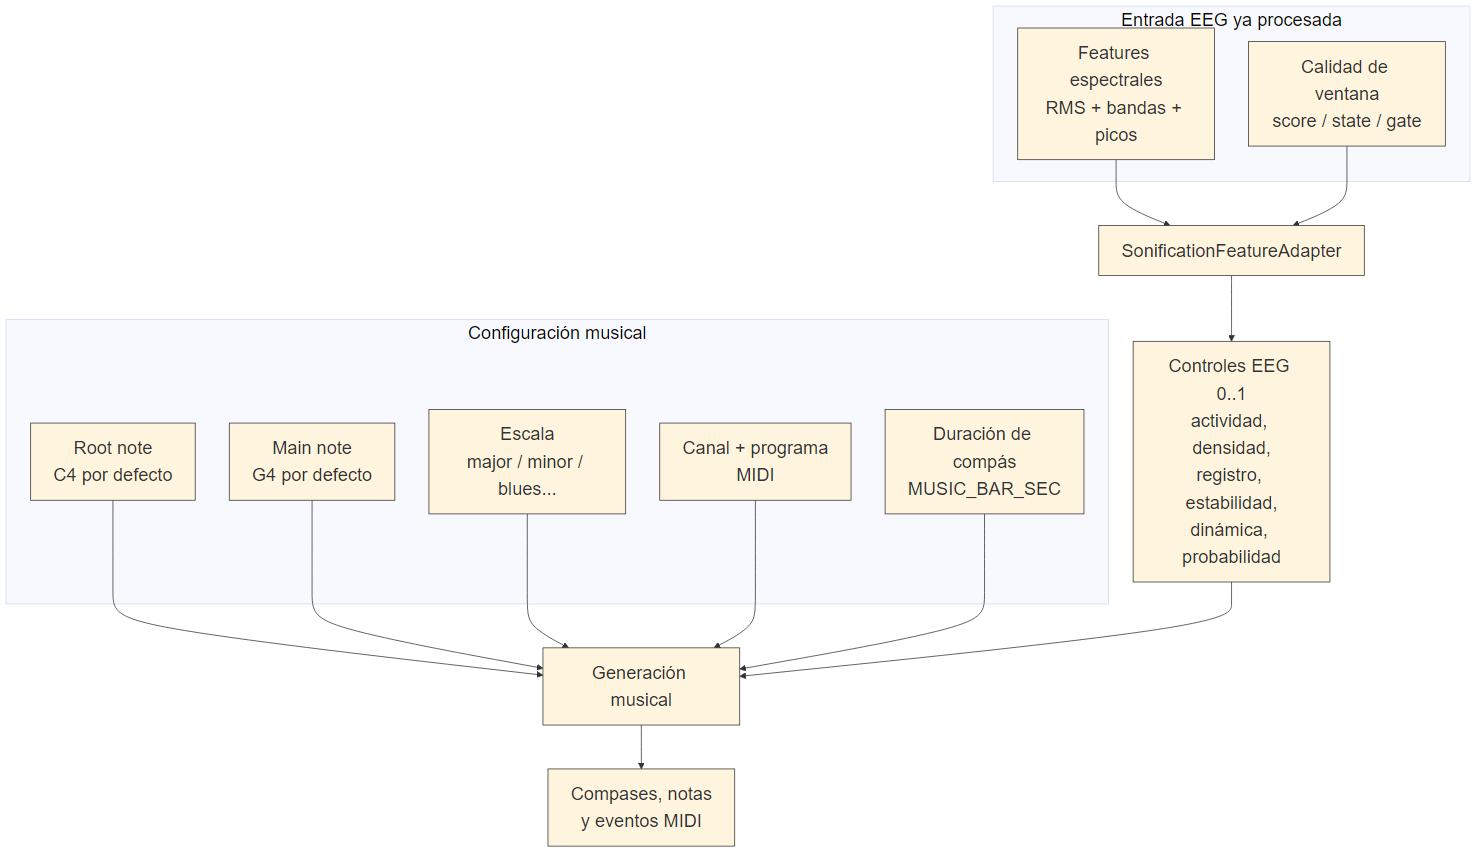
\includegraphics[width=0.95\textwidth,height=0.46\textheight,keepaspectratio]{images/uml/impl_sonificacion_controles.png}
    }{%
        \IfFileExists{images/uml/impl_sonificacion_controles.pdf}{%
            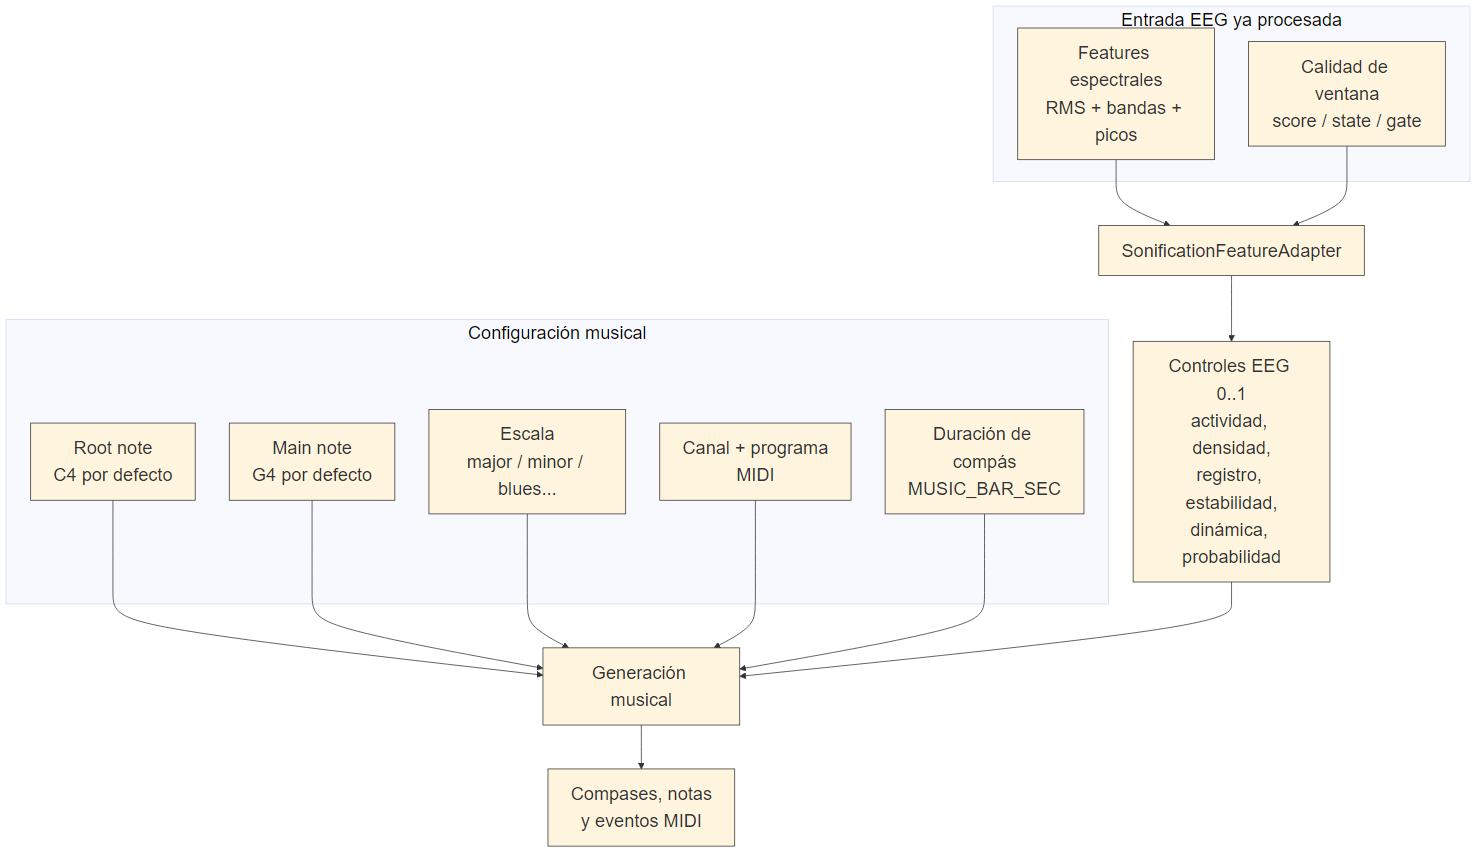
\includegraphics[width=0.95\textwidth,height=0.46\textheight,keepaspectratio]{images/uml/impl_sonificacion_controles.pdf}
        }{%
            \fbox{\parbox{0.9\textwidth}{\centering Diagrama pendiente de exportar desde Mermaid: \texttt{images/uml/impl\_sonificacion\_controles.mmd}}}%
        }%
    }
    \caption{Separación entre características EEG, calidad de señal y configuración musical. El EEG modula controles continuos; la nota raíz, la nota principal, la escala, el canal, el programa y la duración del compás proceden de la configuración musical.}
    \label{fig:impl_sonificacion_controles}
\end{figure}

La construcción de segmentos también permite bloquear la generación si las características no son válidas. En el backend, \texttt{\_maybe\_generate\_music()} no continúa si no existe \texttt{\_last\_sonification} o si el objeto no está marcado como válido. De esta forma, una ventana mala no produce un nuevo compás, aunque puedan quedar eventos MIDI ya programados desde una ventana anterior.

\subsubsection{Generación de compases}

El siguiente nivel de la jerarquía es el compás. \texttt{BarGenerator} recibe un \texttt{MusicSegment} y produce un objeto \texttt{Bar}. Este objeto contiene el índice del compás, tiempos de inicio y fin, la raíz del acorde, las notas del acorde, un patrón de posiciones activas y una envolvente musical sintética. El compás funciona como puente entre controles continuos y notas individuales.

La implementación usa una cuadrícula de 16 posiciones por compás: cuatro pulsos con cuatro subdivisiones por pulso. Cada posición puede estar activa o en silencio. El primer slot se fuerza como ancla musical para que el compás tenga un punto de referencia estable. El número objetivo de notas depende de la cadencia rítmica \texttt{LOW}, \texttt{MEDIUM} o \texttt{HIGH}, y se ajusta ligeramente con la actividad estimada.

Los pesos de selección de slots combinan reglas musicales y controles EEG. La base favorece el primer pulso, los tiempos principales y ciertas subdivisiones. Después, la actividad incrementa la probabilidad global de eventos, la tensión favorece síncopas u \textit{offbeats}, y \texttt{band\_note\_probability} ajusta la probabilidad general de activar posiciones. Por tanto, el EEG no decide manualmente cada slot, sino que modifica una distribución musical ponderada.

En paralelo, el compás selecciona un acorde diatónico a partir de la escala activa. La estabilidad armónica y la tensión determinan si se tiende a un grado estable, intermedio o de mayor tensión. La implementación utiliza histéresis armónica para evitar saltos continuos entre grados por cambios pequeños de la señal. Esto mantiene una salida más coherente en tiempo real.

La Figura~\ref{fig:impl_sonificacion_segmento_compas_nota} resume la relación entre segmento, compás y notas. La misma figura se utiliza también como guía para la subsección siguiente, porque muestra que las notas se generan después de disponer de escala, acorde, patrón rítmico y controles musicales.

\begin{figure}[H]
    \centering
    \IfFileExists{images/uml/impl_sonificacion_segmento_compas_nota.png}{%
        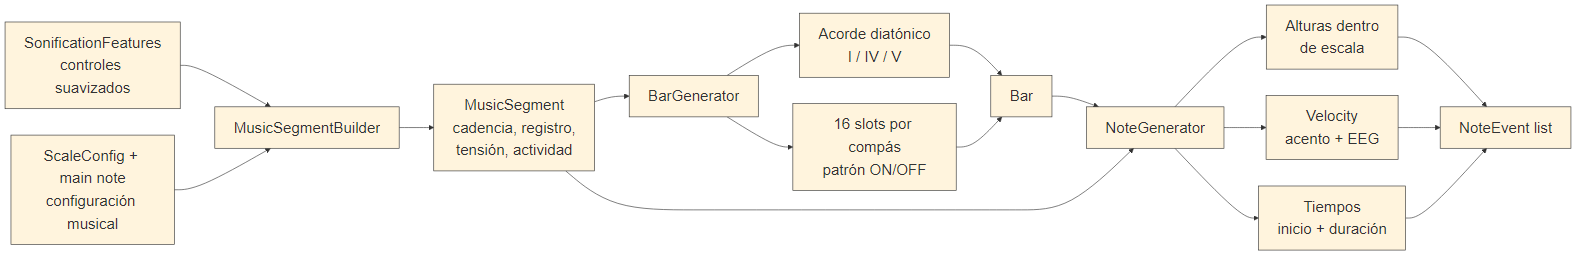
\includegraphics[width=0.98\textwidth,height=0.46\textheight,keepaspectratio]{images/uml/impl_sonificacion_segmento_compas_nota.png}
    }{%
        \IfFileExists{images/uml/impl_sonificacion_segmento_compas_nota.pdf}{%
            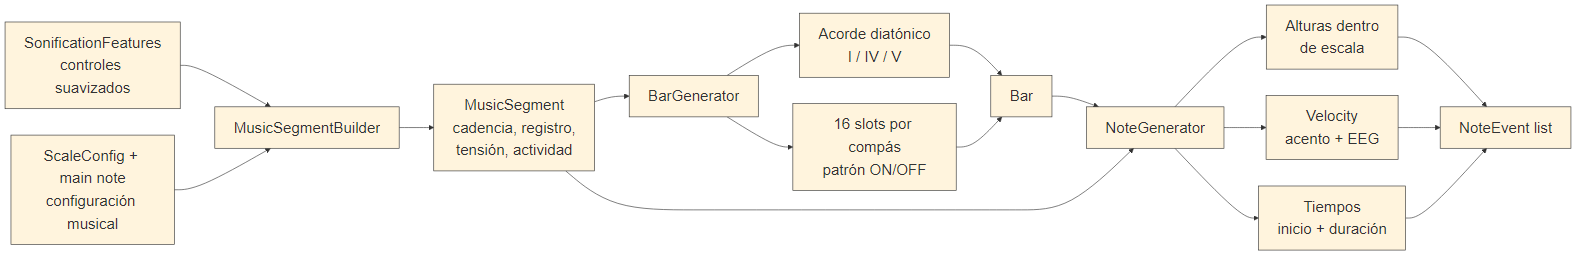
\includegraphics[width=0.98\textwidth,height=0.46\textheight,keepaspectratio]{images/uml/impl_sonificacion_segmento_compas_nota.pdf}
        }{%
            \fbox{\parbox{0.9\textwidth}{\centering Diagrama pendiente de exportar desde Mermaid: \texttt{images/uml/impl\_sonificacion\_segmento\_compas\_nota.mmd}}}%
        }%
    }
    \caption{Jerarquía musical empleada por la sonificación. Los controles EEG suavizados y la configuración musical construyen un segmento; el segmento genera un compás con acorde y patrón rítmico; el generador de notas produce eventos \texttt{NoteEvent}.}
    \label{fig:impl_sonificacion_segmento_compas_nota}
\end{figure}

\subsubsection{Generación de notas}

\texttt{NoteGenerator} convierte el \texttt{MusicSegment} y el \texttt{Bar} en una lista de \texttt{NoteEvent}. Esta estructura representa una nota musical de alto nivel, pero todavía no es un mensaje MIDI. Cada \texttt{NoteEvent} contiene tiempo de inicio, tiempo de fin, altura MIDI, \textit{velocity}, canal y programa. La conversión a \texttt{note\_on} y \texttt{note\_off} se realiza después, en el scheduler MIDI.

La selección de alturas se realiza dentro de la escala configurada. Primero se calcula un centro de registro alrededor de la nota principal. El control \texttt{spectral\_register} desplaza suavemente ese centro hacia registros más graves o más agudos, pero la nota principal sigue actuando como referencia musical. A partir de ese centro se construye un conjunto de notas de la escala dentro de un radio determinado, y se separan notas de acorde y notas de paso.

Las posiciones fuertes del compás tienden a utilizar notas del acorde, mientras que las posiciones intermedias pueden usar notas de paso cuando existen candidatos adecuados. La tensión EEG desplaza el objetivo melódico y puede permitir intervalos algo mayores, mientras que la actividad y la probabilidad influyen en la variedad. Aun así, el generador limita los saltos respecto a la nota anterior para evitar melodías erráticas y mantiene las alturas dentro del rango MIDI permitido.

La dinámica se calcula mediante la función de \textit{velocity}. Esta combina un acento musical base según la posición rítmica, el factor EEG \texttt{rms\_band\_velocity} y la envolvente sintética del compás. El resultado se acota entre una velocidad mínima y máxima para evitar notas demasiado débiles o excesivamente agresivas. En este punto, el EEG afecta a la intensidad y al carácter de la nota, pero no se interpreta como una medida clínica de activación cerebral.

La duración de cada nota se obtiene a partir de la cuadrícula del compás. Una nota dura hasta el siguiente slot activo o hasta el final del compás. Si por seguridad se detectara una duración nula o negativa, se impone una duración mínima. Esta regla es importante para el flujo MIDI posterior, porque cada nota debe tener un inicio y un final definidos para evitar notas colgadas.

En el primer slot, el sistema puede generar el acorde completo como marcador armónico. El backend decide si se reproduce ese acorde completo según un periodo mínimo y según si los controles musicales han cambiado de forma suficiente. Así se evita que cada compás repita un acorde completo de forma innecesaria, manteniendo una textura más ligera cuando el estado EEG no cambia significativamente.

\subsubsection{Escritura y transmisión MIDI}

La escritura MIDI se divide en dos niveles. El primer nivel es musical y trabaja con \texttt{NoteEvent}; el segundo nivel es MIDI y trabaja con eventos temporizados y bytes. Esta separación permite que \texttt{NoteGenerator} no tenga que conocer el transporte físico, y que \texttt{MidiByteTransport} no tenga que conocer las reglas de generación musical.

\texttt{MidiScheduler}, implementado en \texttt{midi\_live.py}, transforma cada \texttt{NoteEvent} en dos eventos MIDI vivos: un \texttt{note\_on} en el inicio de la nota y un \texttt{note\_off} en su final. Además, el backend programa un \texttt{program\_change} una sola vez al inicio para fijar el programa MIDI de salida. Los eventos se almacenan en una cola temporal ordenada por \texttt{due\_time}, usando el reloj monotónico del sistema.

En cada iteración del backend, \texttt{\_pump\_midi()} llama a \texttt{pop\_due\_events(now, lookahead\_sec=MIDI\_LOOKAHEAD\_SEC)}. El \textit{lookahead} de \SI{0.02}{\second} permite extraer eventos ligeramente por adelantado, de modo que el transporte y el firmware dispongan de margen para emitirlos sin bloquear el ciclo principal. El scheduler no envía nada por sí mismo: solo decide qué eventos están vencidos o próximos a vencer.

La conversión a bytes se realiza mediante \texttt{event\_to\_midi\_bytes()}. Un \texttt{note\_on} se codifica con estado \texttt{0x90 | channel}, nota y \textit{velocity}; un \texttt{note\_off} usa \texttt{0x80 | channel}; un \texttt{control\_change} usa \texttt{0xB0 | channel}; y un \texttt{program\_change} usa \texttt{0xC0 | channel}. Todos los canales se limitan a 0--15 y los datos MIDI a 0--127.

\texttt{MidiByteTransport} recibe los eventos vencidos, los convierte en bytes y llama al \textit{handler} del firmware mediante \texttt{Bridge.call("midi\_bytes", n, b0, b1, b2)}. El campo \texttt{n} indica si el mensaje tiene dos o tres bytes válidos. El firmware no decide qué nota tocar ni interpreta musicalmente el mensaje: recibe los bytes y los escribe por la UART asociada a la salida MIDI física.

La salida física validada usa \texttt{Serial1}/D1 a la velocidad MIDI estándar de \SI{31250}{baudios}, con transmisión invertida en el microcontrolador. Esta configuración pertenece a la capa de firmware y electrónica ya descrita previamente; en 6.3 basta con indicar que la ruta Python--Bridge--firmware desemboca en esa UART física y, desde ella, en el conector MIDI OUT del prototipo.

La Figura~\ref{fig:impl_midi_eventos_bytes} resume la formación de mensajes MIDI desde las notas generadas. Esta figura aclara la diferencia entre nota musical, evento MIDI temporizado, bytes MIDI y transporte físico.

\begin{figure}[H]
    \centering
    \IfFileExists{images/uml/impl_midi_eventos_bytes.png}{%
        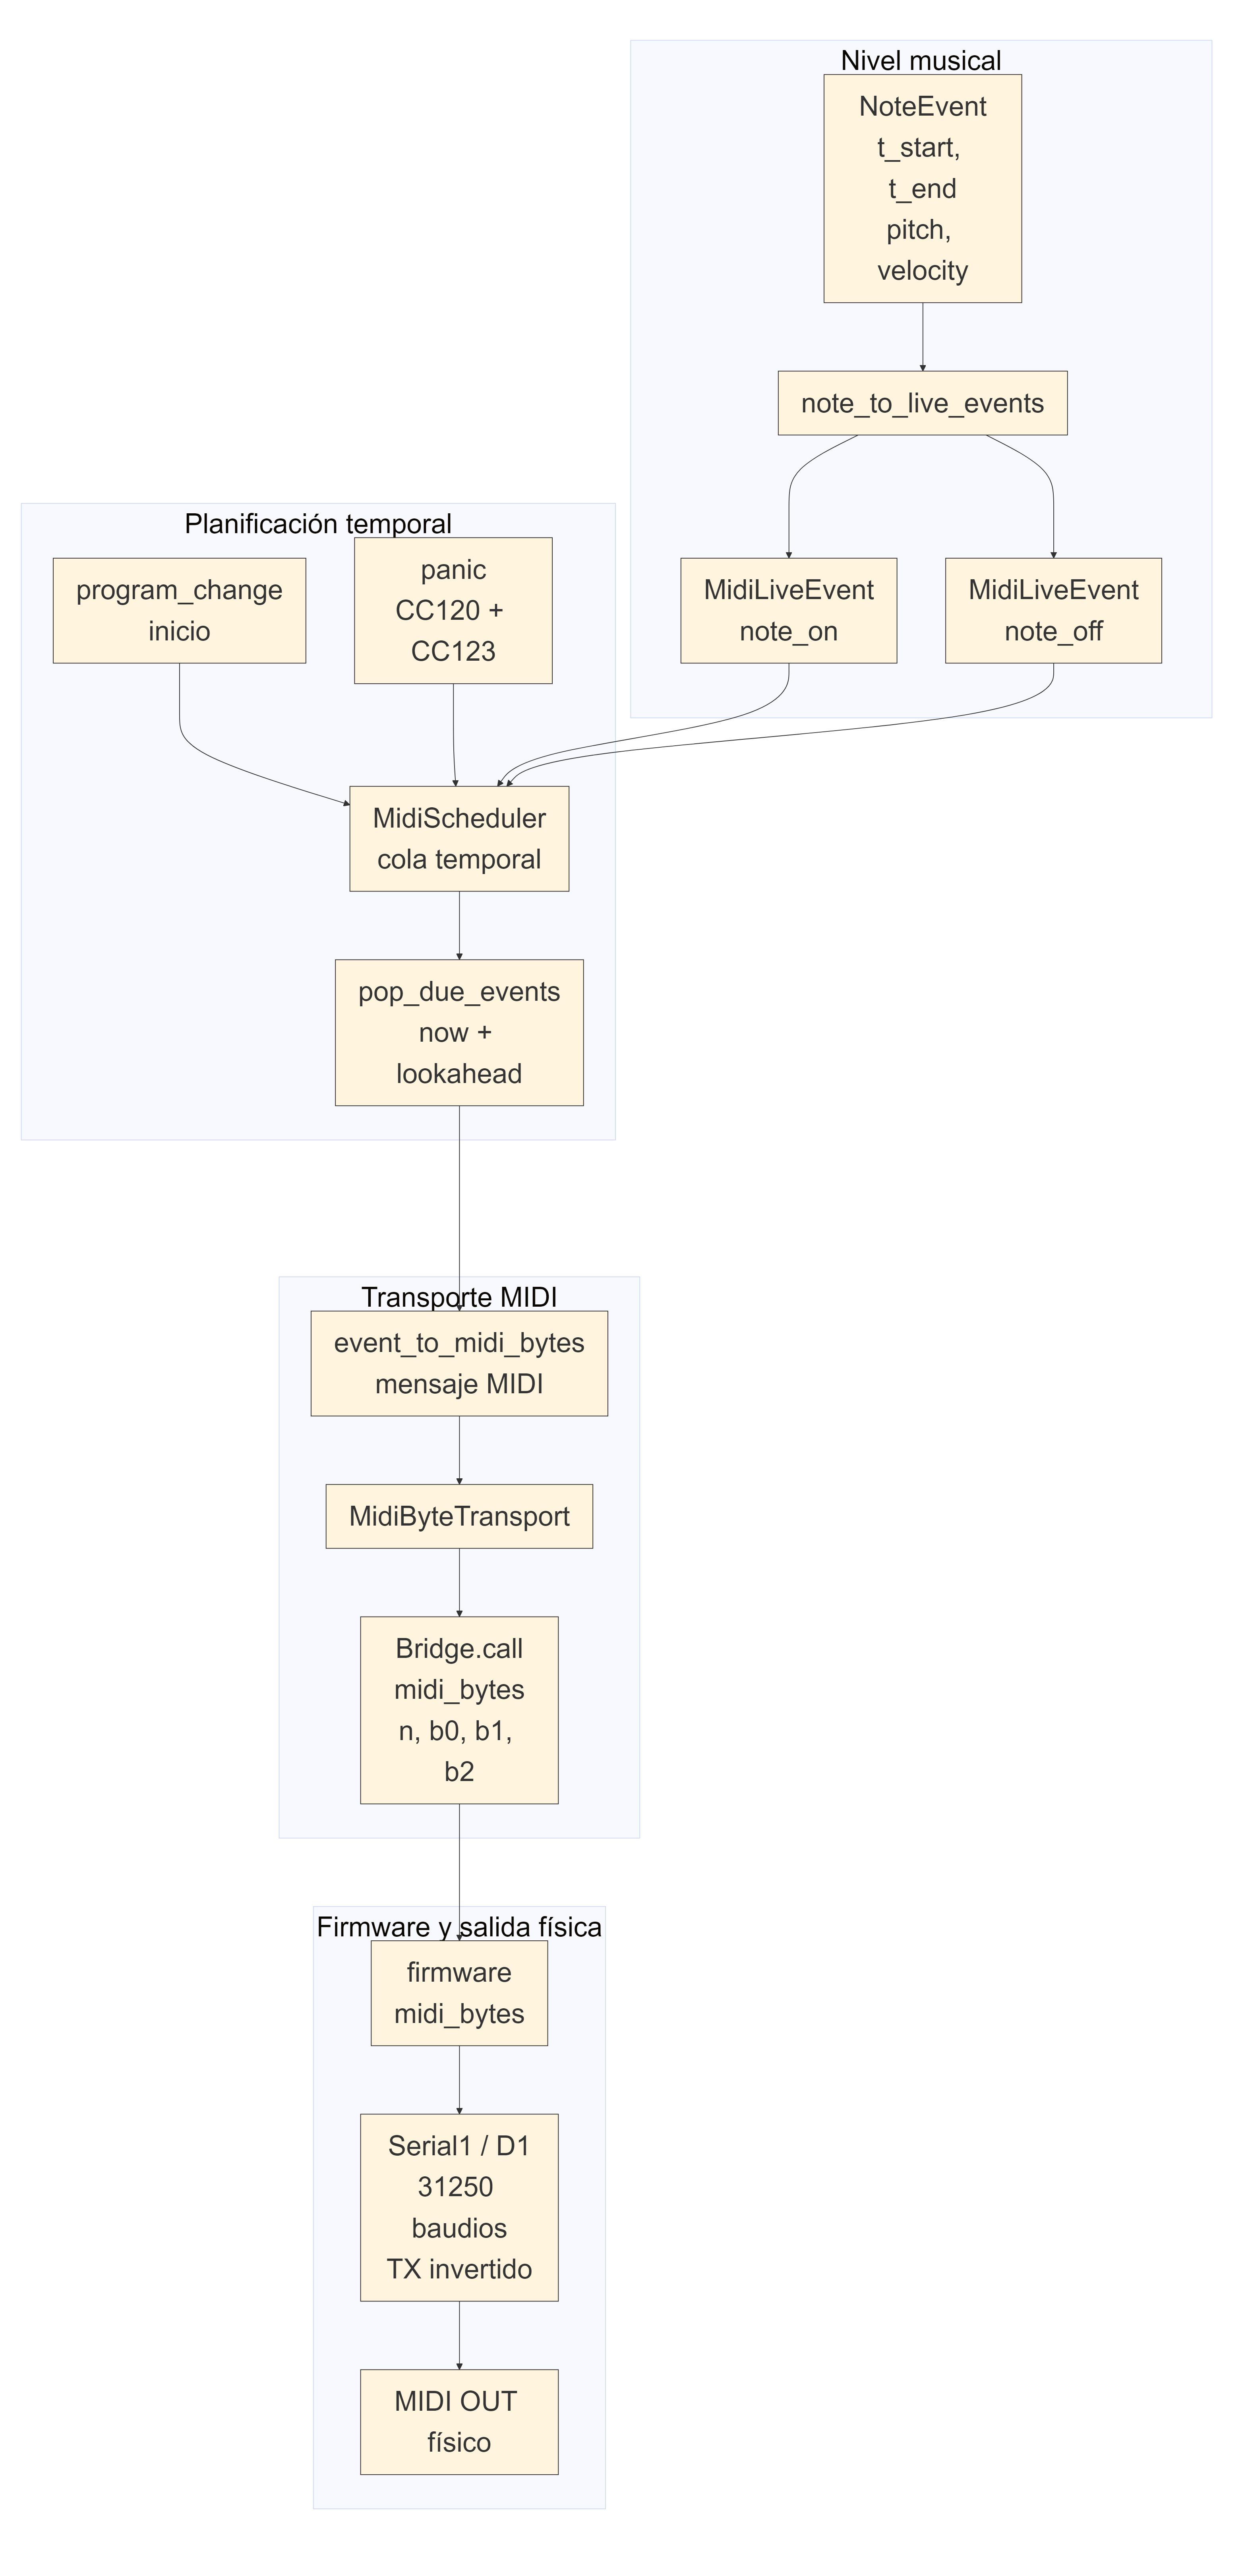
\includegraphics[width=0.98\textwidth,height=0.46\textheight,keepaspectratio]{images/uml/impl_midi_eventos_bytes.png}
    }{%
        \IfFileExists{images/uml/impl_midi_eventos_bytes.pdf}{%
            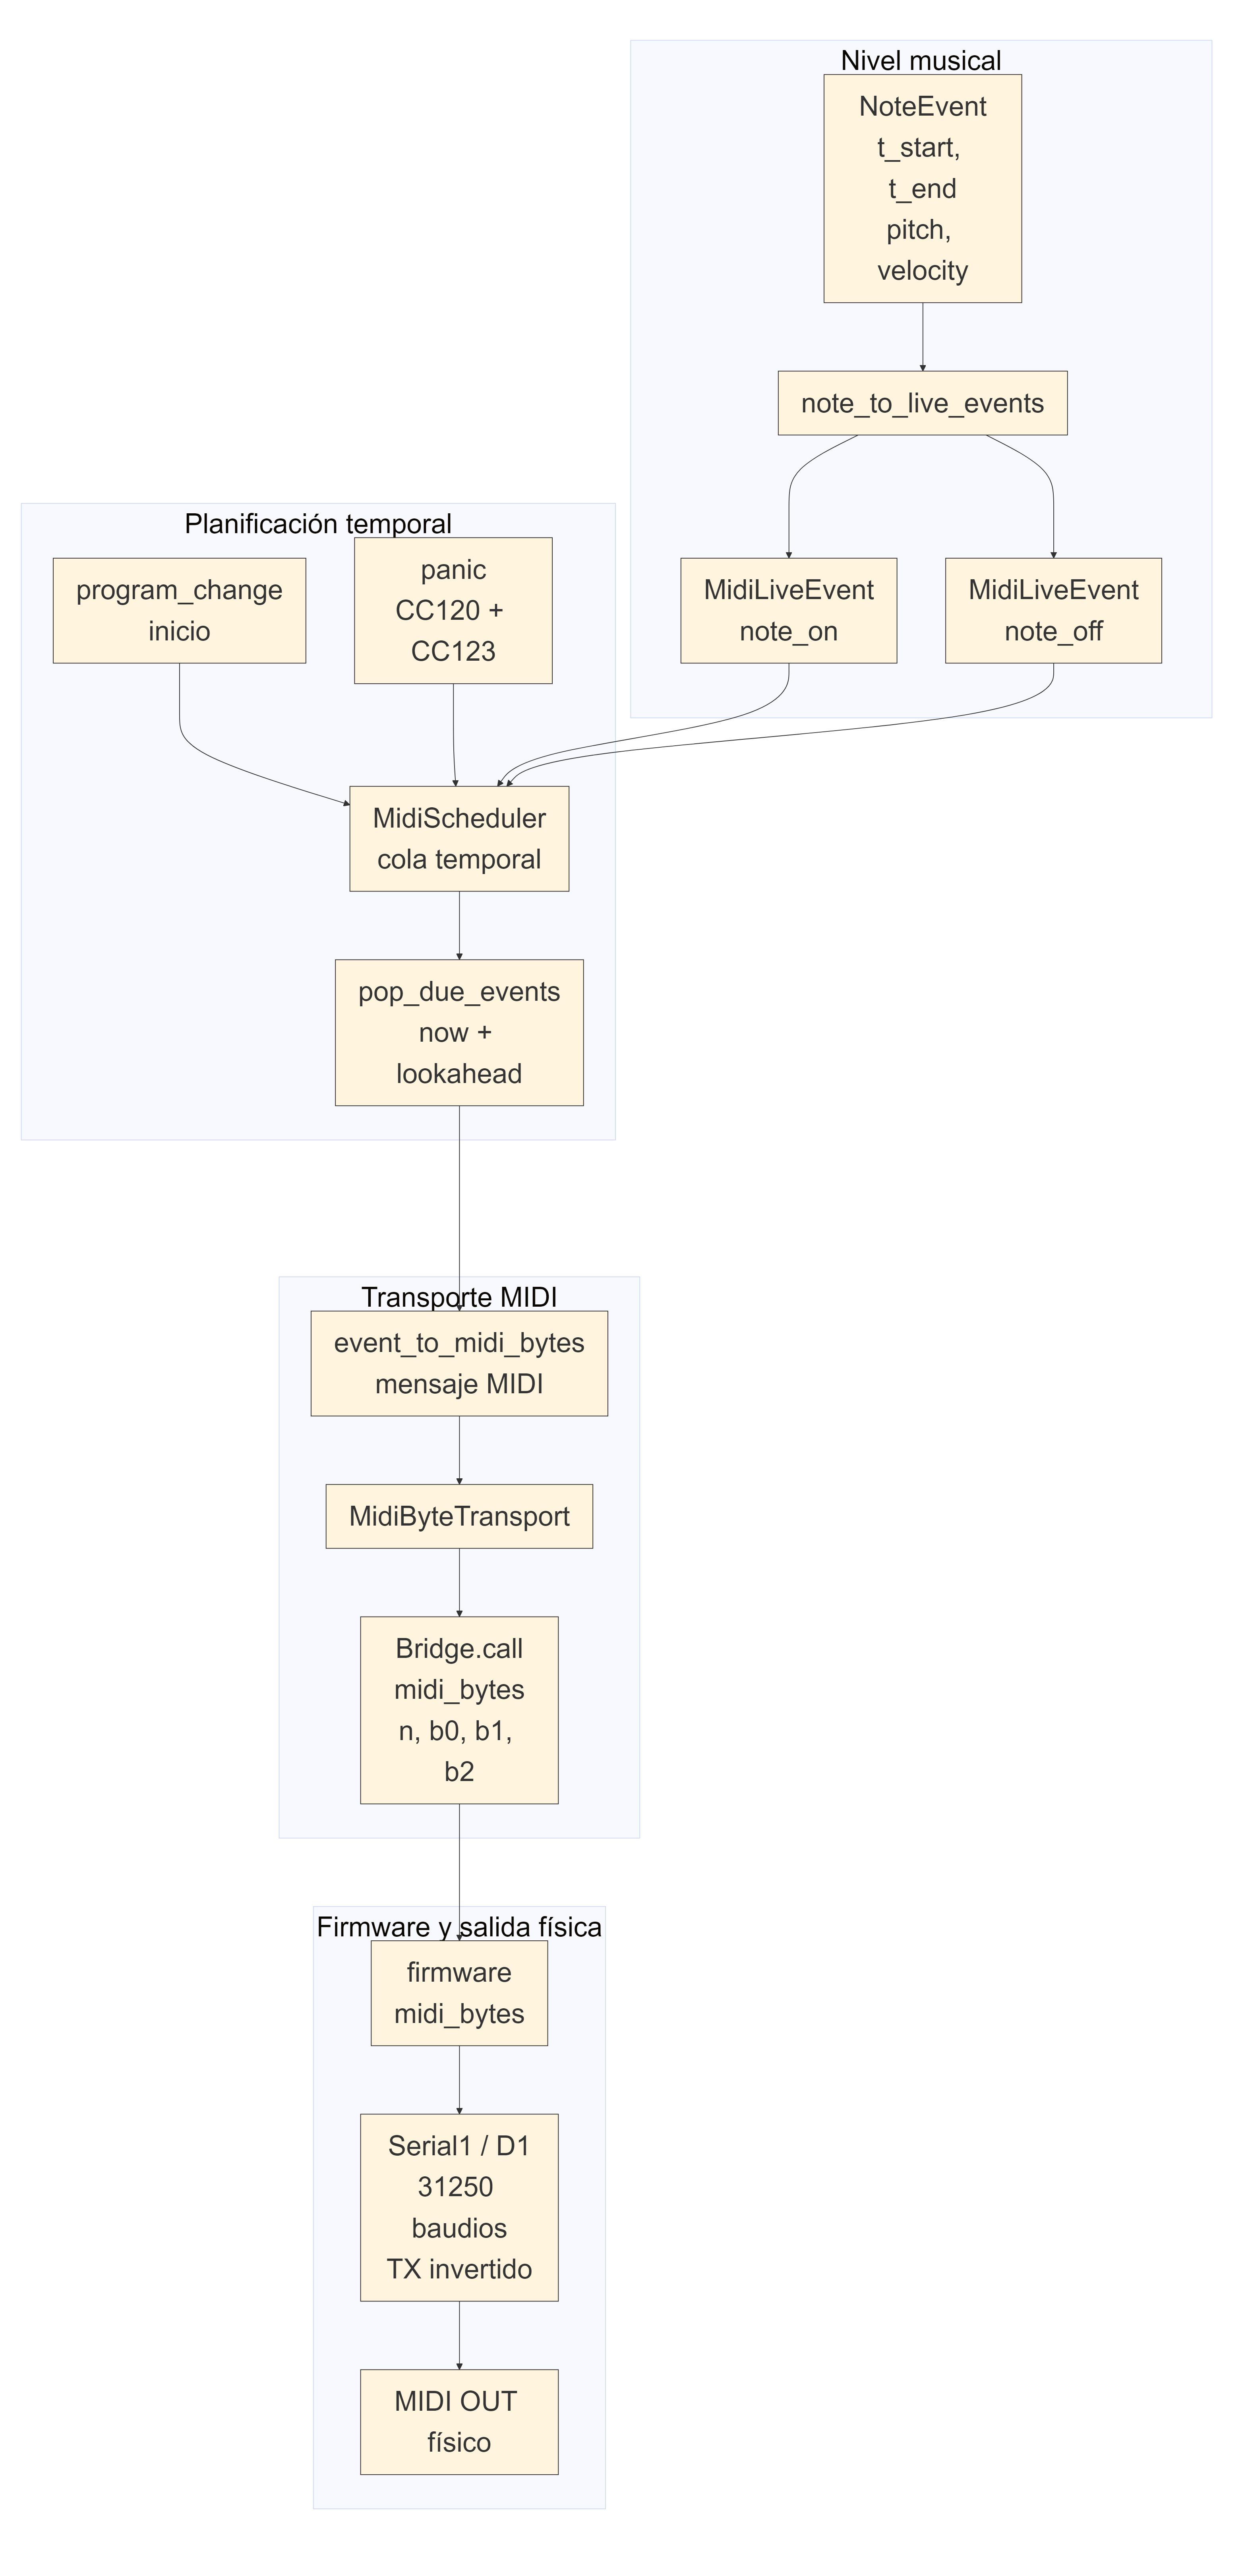
\includegraphics[width=0.98\textwidth,height=0.46\textheight,keepaspectratio]{images/uml/impl_midi_eventos_bytes.pdf}
        }{%
            \fbox{\parbox{0.9\textwidth}{\centering Diagrama pendiente de exportar desde Mermaid: \texttt{images/uml/impl\_midi\_eventos\_bytes.mmd}}}%
        }%
    }
    \caption{Formación de mensajes MIDI en la ruta live. Las notas de alto nivel se transforman en eventos \texttt{note\_on}, \texttt{note\_off} y \texttt{program\_change}; después se convierten a bytes y se envían al firmware mediante \texttt{midi\_bytes}.}
    \label{fig:impl_midi_eventos_bytes}
\end{figure}

Como medida de seguridad, el sistema conserva la ruta \texttt{panic}. Esta acción limpia el scheduler y genera mensajes \texttt{All Sound Off} y \texttt{All Notes Off} para todos los canales. Es necesaria porque una ventana de mala calidad puede bloquear la generación de nuevos compases, pero no elimina automáticamente eventos que ya hubieran sido programados desde una ventana anterior. Por tanto, el \textit{panic} forma parte de la robustez del sistema MIDI y debe mantenerse aunque se simplifique la lógica musical.

La salida MIDI puede desactivarse mediante la variable de entorno \texttt{EEG\_MIDI\_LIVE\_ENABLED}. En ese caso, los eventos pueden seguir generándose y contabilizándose, pero el transporte los marca como descartados en lugar de enviarlos al firmware. Esta opción permite validar generación y scheduler sin forzar siempre el envío físico por la UART MIDI.
